\documentclass[11pt]{article}
\usepackage[a4paper,margin=2.5cm]{geometry}
\usepackage[T1]{fontenc}
\usepackage{booktabs}
\usepackage{graphicx}
\usepackage{hyperref}
\usepackage{natbib}
\usepackage{tabularx}

\title{Lost in Roman Urdu: Small Local Language Models Drop Red Flags,\\ Body Parts and Laterality When Drafting Physiotherapy Notes}
\author{Muzammal Hussain\\Masmatix Innovations, Glasgow, United Kingdom\\\texttt{muzammal@masmatixinnovations.co.uk}}
\date{Draft, October 2026}

\begin{document}
\maketitle

\begin{abstract}
Small language models that run on a clinic's own computer are attractive for drafting clinical notes, because patient speech never leaves the building. In Pakistan and in UK clinics serving Pakistani communities, many consultations are held in Roman Urdu: Urdu written in Latin script and mixed with English clinical terms. We ask whether two small local models, Qwen2.5 3B and Llama 3.1 8B, write English SOAP notes from Roman Urdu consultations as safely as from English ones. We wrote 20 fictional physiotherapy consultations, each in English and Roman Urdu with identical facts, listed 168 facts (68 critical) and checked every note automatically for omissions, wrong body regions and the injured side. From Roman Urdu, Llama 3.1 8B omitted 16 of 168 facts against 1 from English (exact McNemar $p=0.0003$) and Qwen2.5 3B omitted 50 against 6 ($p<0.0001$). Critical facts were lost only in Roman Urdu (8 and 26). The injured side was missing from 13 and 14 of the 14 Roman Urdu notes where a side applied, and reading the notes showed a knee replacement rewritten as a hip replacement, a hip as the lower back, and left as right. In a four-case pilot, translating into English before drafting did not help. A simple rule-based gate flagged 17 of 20 Llama 3.1 8B Roman Urdu notes and none of its English notes. All consultations, notes and code are public.
\end{abstract}

\section{Introduction}
Large language models can turn a consultation into a structured note, but they also leave facts out and add facts that were never said. \citet{asgari2025framework} measured this for GPT-4 on 450 simulated UK primary-care consultations and found a 1.47\% hallucination rate and a 3.45\% omission rate, with most major errors in the Plan. Their study used one large hosted model and English only.

Two practical settings fall outside that study. First, many clinics cannot send recordings to a hosted model, so the relevant models are small ones that run locally. Second, a large share of consultations in Pakistan, and among Pakistani patients in the UK, take place in Roman Urdu, which is rarely represented in clinical evaluation data.

This paper reports a controlled comparison: the same consultations, the same facts and the same prompt, once in English and once in Roman Urdu, drafted by two small local models. Our contributions are:
\begin{itemize}
  \item a public set of 20 paired English and Roman Urdu physiotherapy consultations with 168 listed facts, 68 marked critical, including deliberate red flags;
  \item a paired comparison showing that both models lose significantly more facts, and only lose critical facts, in Roman Urdu;
  \item an analysis of anatomy and laterality errors, showing that the injured side is almost never carried into the English note;
  \item a negative result for translating first, and a simple rule-based gate that routes notes to a clinician.
\end{itemize}

\section{Data and method}
\paragraph{Consultations.} The author wrote 20 short fictional physiotherapy consultations (back, neck, shoulder, knee, hip and pelvis, ankle and foot, wrist and hand, elbow). Each exists in English and Roman Urdu with the same facts and numbers. Clinical terms that clinicians in Pakistan normally say in English (for example ligament, ACL, scaphoid) stay in English inside the Roman Urdu, as in real code-mixed speech. Several cases contain red flags on purpose: saddle numbness with urinary difficulty (suspected cauda equina syndrome), a swollen calf two weeks after knee replacement (possible deep vein thrombosis), weight loss with a history of cancer, and a possible scaphoid fracture in a patient on warfarin. No real patient data was used.

\paragraph{Facts.} Each consultation lists 6 to 11 facts with a keyword pattern; 68 of 168 are marked critical (red-flag answers, medicines, referrals and urgent actions). Every pattern is tested to match its own English transcript. Fourteen cases have an injured side.

\paragraph{Models and prompt.} Qwen2.5 3B \citep{qwen2025qwen25} and Llama 3.1 8B \citep{grattafiori2024llama3} ran through Ollama on a MacBook M4 with 16\,GB memory, at temperature 0 with a fixed seed. The system prompt asked for a concise English SOAP note with four headings, using only information in the transcript. This gives 80 notes.

\paragraph{Checks.} For each note we record (i) listed facts whose pattern is absent, (ii) whether the main body region is named, (iii) body regions named in the note but absent from the English transcript, (iv) whether the injured side is named, and (v) whether the opposite side is named without support. A note is \emph{flagged} for clinician review if any of (ii) to (v) fails or a critical fact is missing.

\paragraph{Statistics.} We report the facts-missing rate with a 95\% bootstrap interval that resamples whole consultations \citep{efron1979bootstrap}, and an exact two-sided McNemar test \citep{mcnemar1947} on each fact paired across languages.

\section{Results}
\begin{table}[t]
\centering
\small
\begin{tabular}{llrrrrr}
\toprule
Model & Language & Missing (of 168) & \% (95\% CI) & Critical & Side missing (of 14) & Flagged (of 20)\\
\midrule
Qwen2.5 3B & English & 6 & 3.6 (1.2--6.2) & 0 & 0 & 3\\
Qwen2.5 3B & Roman Urdu & 50 & 29.8 (24.0--35.4) & 26 & 14 & 20\\
Llama 3.1 8B & English & 1 & 0.6 (0.0--1.8) & 0 & 0 & 0\\
Llama 3.1 8B & Roman Urdu & 16 & 9.5 (5.6--13.9) & 8 & 13 & 17\\
\bottomrule
\end{tabular}
\caption{Omissions, side and gate results for 20 consultations per language.}
\label{tab:main}
\end{table}

\begin{figure}[t]
\centering
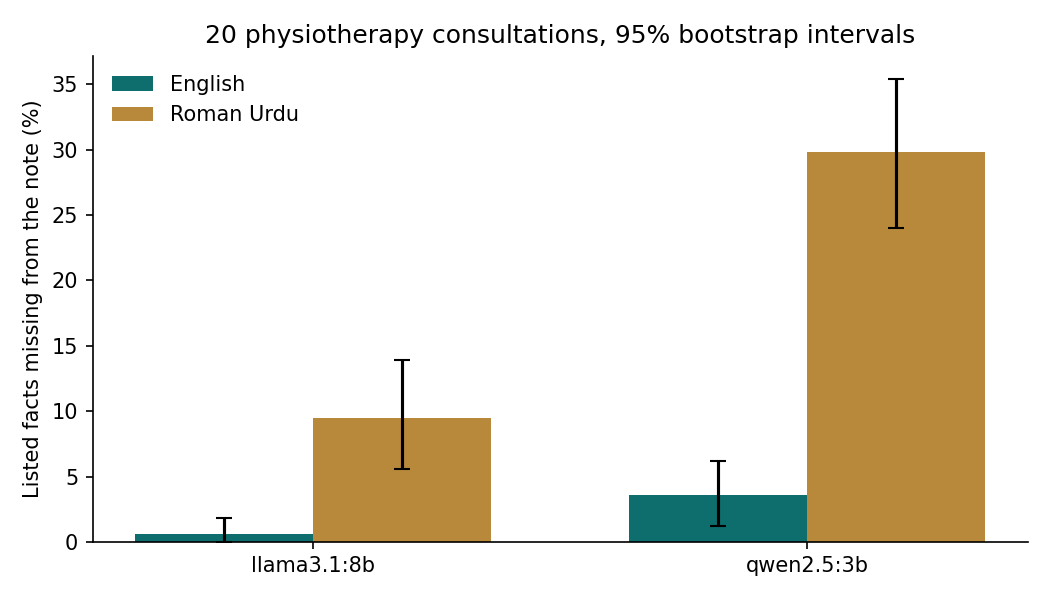
\includegraphics[width=0.72\linewidth]{figures/facts_missing_by_language.png}
\caption{Share of listed facts missing, with 95\% bootstrap intervals over consultations.}
\label{fig:main}
\end{figure}

\paragraph{Omissions.} Table~\ref{tab:main} and Figure~\ref{fig:main} show the main result. For Llama 3.1 8B, 16 facts were missing only in Roman Urdu and 1 only in English ($p=0.0003$); for critical facts the split was 8 to 0 ($p=0.0078$). For Qwen2.5 3B the splits were 47 to 3 and 26 to 0 (both $p<0.0001$). The larger model narrows the gap but does not close it.

\paragraph{Anatomy and laterality.} The main body region was wrong or missing in 6 Llama 3.1 8B and 11 Qwen2.5 3B Roman Urdu notes. The injured side was dropped almost always: \emph{daayan} (right) and \emph{baayan} (left) were not translated, and Llama 3.1 8B turned left into right twice. Table~\ref{tab:errors} lists errors found by reading the notes.

\begin{table}[t]
\centering
\small
\begin{tabularx}{\linewidth}{lXX}
\toprule
Model & What was said & What the note said\\
\midrule
Llama 3.1 8B & left knee replaced two weeks ago, left calf swollen & ``hip replacement surgery'', pain in the hip; calf not mentioned\\
Llama 3.1 8B & \emph{baayan koolha} (left hip) & ``osteoarthritis of the lower back''\\
Qwen2.5 3B & \emph{baayan koolha} (left hip) & knee pain\\
Llama 3.1 8B & \emph{daayan ghutna} (right knee) & ``a strain to the ankle''\\
Llama 3.1 8B & fall on the left hand & ``grip strength in the right hand''\\
Qwen2.5 3B & saddle numbness, difficulty passing urine & numbness not mentioned; added ``difficulty in defecation'' and ``a 45-year-old male''\\
Llama 3.1 8B & neck stiff and sore after a car accident & ``with a headache'' (never said)\\
\bottomrule
\end{tabularx}
\caption{Errors in Roman Urdu notes found by reading them.}
\label{tab:errors}
\end{table}

The knee replacement case shows why this matters. After knee surgery a swollen calf is the main warning sign of a deep vein thrombosis. The note still raised a possible clot and sent the patient to hospital, but with the wrong joint and without the sign that explains the concern.

\paragraph{Does translating first help?} On the first four consultations we also asked each model to translate the Roman Urdu into English and then draft from its own translation. Qwen2.5 3B returned the Roman Urdu unchanged in all four cases, so the step did nothing. For Llama 3.1 8B, critical facts missing rose from 3 (direct) to 5 (translate first) of 42 facts, and the translation itself swapped a left neck rotation to the right and turned a shoulder into the lower back. This pilot is small, but it gives no support for translation as a fix.

\paragraph{The gate.} The rule-based gate flagged 17 of 20 Llama 3.1 8B Roman Urdu notes and none of its English notes; 5 of the 17 were flagged only for a missing side. Two of the three Qwen2.5 3B English flags were fair wording rather than errors (``calf exercises'' for an ankle sprain, ``right leg'' for a right knee).

\section{Discussion}
For a clinic using these models, the results point to three design rules. First, Roman Urdu notes from small local models cannot be used without a clinician reading the whole note. Second, the side and body region should be checked in code: if the transcript names a side, a note without one should be rejected or marked incomplete. Third, every step of a pipeline needs its own check, as the silent no-op translation shows.

\section{Limitations}
The consultations are fictional, written by one person, and short; real consultations are longer, noisier and come through speech recognition, which adds its own errors \citep{radford2023whisper}. Each model ran once at temperature 0. The checks are keyword based: a fact in unexpected words counts as missing, and a fact stated wrongly can still count as present. Sentence-level hallucinations were not labelled in this study, and the automatic checks have not yet been validated against a physiotherapist's reading of every note. Roman Urdu spelling varies between speakers.

\section{Data and code availability}
All consultations, fact lists, notes, checks and analysis scripts are available at \url{https://github.com/MHKhan50/agentic-ai-research-log} (folders \texttt{clinical-note-hallucination}, \texttt{translate-then-draft} and \texttt{roman-urdu-soap-benchmark}).

\bibliographystyle{plainnat}
\bibliography{refs}
\end{document}
